\documentclass{swp}
\usepackage{hyperref}
\usepackage{amsmath}
\usepackage{amssymb}

\begin{document}

\maketitle{Entwurfsbeschreibung Gesamtprojekt}{13.07.2015}{Martin Lechner}
\\\\\\\\\\

\tableofcontents
%\newpage
\section{Allgemeines}
Die Stadtteilplattform Leipziger Osten soll mit umfangreichen Funktionen ausgestattet sein, um gute Nutzbarkeit zu gew\"ahrleisten. Akteure haben hier die M\"oglichkeit, ein \"offentliches Profil zu erstellen, ihre Veranstaltungen einzutragen und auf einer anschaulichen Karte und einem Terminkalender mit vielen Filterfunktionen der \"Offentlichkeit anzeigen zu lassen. Dadurch soll der Stadtteil Leipziger Osten attraktiver gemacht und Bausteine f\"ur Synergien einzelner Akteure gebildet werden. Diese grundlegende Struktur der Plattform wird auf Basis von Drupal realisiert. Dies erm\"oglicht einen einfachen Ausbau der Webseite mittels Modulen, die f\"ur Drupal zu Verf\"ugung stehen. Neben den vorhandenen werden auch eigene Module entwickelt, beispielsweise um die benutzten Module (Kalender, Karte) mit der Datenstruktur zu verkn\"upfen.\\
Die Plattform entsteht in Zusammenarbeit mit Matthias Petzold von leipziger-ecken.de und orientiert sich an ihrem Konzept f\"ur eine Stadtteil-Internetseite.
\subsection{Installationsanleitung}
Drupal muss auf einem Webserver installiert werden. Anweisungen hierf\"ur sind unter \url{https://www.drupal.org/documentation/install} zu finden. Bei erfolgreicher Installation m\"ussen die Drupal-Module: XXX installiert werden. Es wird ein eigenst\"andiges Modul (aae\_{}data) und Thema (aae\_{}theme) entwickelt, so dass diese lediglich in den entsprechenden Drupal-Ordner kopiert und via Backend aktiviert werden m\"ussen. Dabei wird die Datenstruktur in die Datenbank importiert, sowie Inhalte (Akteure, Events, Geodaten) von KILO in die Datenbank geladen. Diese Daten liegen im JSON-Format vor.  Plattforminterne Inhalte k\"onnten \"uber ein Datenbank-Dump erfolgen, welche als Datei im SQL-Format bereit gestellt wird. Externe Inhalte von Leipzig Open Data k\"onnten \"uber eine Funktion im Backend bzw. mittels t\"aglicher CRON-Jobs in die Datenbank integriert werden.
\subsection{Backupkonzept}
Um ein sicheres Arbeiten zu gew\"ahrleisten, wird nicht auf der Drupalinstanz des Servers gearbeitet. Jedes Teammitglied installiert sich eine eigene Drupalinstanz auf seinem lokalen Arbeitsrechner. Der \glqq core\grqq{} wird dabei nicht ver\"andert, d.h. Originalthemes und -module werden nicht ver\"andert. Sollten wir \"Anderungen vornehmen m\"ussen, dann werden diese in einem abgeleiteten eigenen Modul implementiert, gleiches gilt f\"ur Themes. Die bearbeiteten Module werden \"uber das git-Repository verwaltet und in Drupal verlinkt, so dass Fehlschl\"age r\"uckg\"angig gemacht werden k\"onnen.
\section{Produkt\"ubersicht}
\subsection{Drupal}
Drupal wurde bereits installiert, sowie Bausteine f\"ur die Karte und das Layout gesetzt. F\"ur das Aufsetzen der Website mit den bereits genannten Funktionen (Kalender, Eventseite, Akteurprofil) werden im Hauptprojekt b\"undelweise Module implementiert. Hierbei kann auf vorhandene Module zur\"uckgegriffen werden, welche entsprechend angepasst werden bzw. \"uber ein eigenes Modul miteinander verkn\"upft werden.  Eventseite und Akteurprofil wurden inzwischen \"uber das Projektmodul aae\_{}data implementiert. 
\subsection{Layout}
\subsubsection{Darstellung \"Offentliches Profil}
Ein \"offentliches Profil beinhaltet zentrale Informationen zum Akteur (Name, Adresse, E-Mail, Webseite, Telefonnummer, Beschreibung) und eventuell Bild- und Videomaterial. Das Profil soll mit den Events, dem Kalender und der interaktiven Karte verkn\"upft werden. Diese soll auf dem Profil ebenso dargestellt werden.
\subsubsection{Darstellung Kalender}
In einem Kalender werden Events zeitlich dargestellt. \"Uber Filteroptionen k\"onnen hierbei \glqq Wunsch-Events\grqq{} angezeigt werden. Von dem Kalender aus sollen die Eventseiten und die \"offentlichen Profile erreichbar sein.
\subsubsection{Darstellung Events}
Events werden auf einer eigenen Seite dargestellt. Diese beinhaltet Name, Datum, Ort, Zielgruppe, Sparte, Beschreibung, die Verkn\"upfung zum \"offentlichen Profil des Erstellers und der Darstellung des Events auf der interaktiven Karte. Die Events sollen \"uber den Kalender, das \"offentliche Profil des Veranstalters und \"uber die \"Ubersichtskarte auf der Startseite erreichbar sein.
\subsubsection{Darstellung Journal}
Das Jounal wird auf einer eigenen Seite dargestellt werden und zeigt Beitr\"age der Redakteure. Diese bestehen aus einem Bild und einem Text.
\subsubsection{Darstellung Interaktive Karte}
Eine interaktiver Karte soll Informationen zu Akteuren und Events ortsbezogen darstellen. Die Darstellung wird mit OpenStreetmap realisiert. Die interaktive Karte sollte sowohl als Ganzes auf einer eigenen Seite pr\"asentiert werden, als auch in entsprechenden Ausschnitten auf den Seiten von Akteuren und Events eingebunden werden. \"Uber Filterm\"oglichkeiten sollen angezeigte Events aussortiert bzw. hervorgehoben werden. Die Darstellung von Ortsangaben auf der Karte sollte weitestgehend automatisch anhand von Veranstaltungs- bzw. Kontaktadressen erfolgen. F\"ur einige Zwecke kann jedoch auch eine manuelle Darstellung durch einen Veranstalter sinnvoll sein, beispielsweise wenn eine Veranstaltung an einem Ort stattfindet, der nicht durch eine Adresse beschreibbar ist: F\"ur bestimmte Orte innerhalb eines Parks w\"are die Eingabe der exakten Koordinaten durch den Veranstalter beim Erstellen des Events die bessere L\"osung. 
\subsection{Inhalte}
Es werden 56 Datens\"atze von Akteuren der K.I.L.O.-Seite in die Datenbank geladen, sowie 17 Events von K.I.L.O.\\
Inhalte von Akteuren au{\ss}erhalb der \"ubergebenen K.I.L.O.-Daten oder des Leipzig Open Datas Projekts m\"ussen von diesen selbst eingetragen werden. 
\subsection{Funktionalit\"aten}
\subsubsection{Nutzerregistrierung}
Ein User hat die M\"oglichkeit sich auf der Plattform zu registrieren, um ein \"offentliches Profil zu erstellen. Von diesem aus kann er Events erstellen, welche, wie das Profil, von Besuchern der Webseite eingesehen werden k\"onnen.
\section{Grunds\"atzliche Struktur- und Entwurfsprinzipien}
\subsection{MVC/PAC-Modell}
F\"ur das Projekt adaptieren wir das MVC-Modell. Im Model werden die Datens\"atze verwaltet. Der Controller reagiert dann auf Nutzeranfragen, wie einer Suche und leitet diese an das Model weiter. Das Model verarbeitet diese Anfrage und gibt das Ergebnis zur Darstellung an den View weiter. Drupal selbst baut auf eine erweiterte Form des MVC-Modells auf. Im Presentation-Abstraction-Control oder PAC Modell entspricht Presentation dem View, und Abstraction dem Model. Im Gegensatz zu MVC findet diese Dreiteilung der Architektur im PAC jedoch f\"ur jeden Systemteil (\glqq Agent\grqq{}) statt, der eine spezifische Aufgabe erf\"ullt. Diesen Agents entsprechen die einzelnen Drupalmodule. Die Kommunikation / Zusammenarbeit dieser stellt einen kritischen Punkt f\"ur das Gelingen des Projekts dar. Dem Controller-Bereich des selbstgeschriebenen Moduls sollte daher besondere Aufmerksamkeit geschenkt werden. Da es im Sinne des PAC-Modells ist, einzelne \glqq Agents\grqq{} f\"ur bestimmte Aufgaben zu haben, sollte eventuell in Betracht gezogen werden, das selbstgeschriebene Modul in mehrere aufzuteilen, sodass es nicht mit verschiedenen Funktionalit\"aten \"uberladen ist.
\subsection{Arbeitsteilung}
Das Team arbeitet in der Implementierungsphase in kleineren Gruppen, um eine parallele aber personell m\"oglichst getrennte Entwicklung von Layout, Backend, und Datenstruktur zu erm\"oglichen.
\subsubsection{Layout}
Der/die Layouter sind mit der Gestaltung der Plattform und ihrer interaktiven Elemente betraut. Das Layout wird fortschreitend mit den anderen Ebenen der Plattform entwickelt, um auf eventuelle \"Anderungen von deren Seiten aus reagieren zu k\"onnen.
\subsubsection{Backend}
Die Backend-Gruppe ist f\"ur die Installation, das Einrichten der Drupal-Instanz verantwortlich. In der Implementierungsphase arbeitet dieser Teil des Teams an der Entwicklung eines eigenen Drupal-Moduls und der Verkn\"upfung aller Module und Funktionalit\"aten des Systems.
\subsubsection{Daten}
Dieser Aufgabenbereich umfasst im aktuellen Fall die Einpflege der oben erw\"ahnten K.I.L.O.-Daten. Dies ist bereits geschehen.
\section{Struktur- und Entwurfsprinzipien einzelner Pakete}
\subsection{Datenebene}
Die K.I.L.O.-Daten stehen im RDF-Format (JSON) zur Verf\"ugung und werden in das Datenmodell unseres Datenbankschemas angepasst.
\subsection{Darstellungsebene}
Es soll eine Hauptseite geben, die die interaktive Karte, den Kalender, Snippets von Akteurprofilen und eine Navigationsleiste beinhaltet. Weiterhin soll es Seiten geben f\"ur: Akteurprofile, Events, den Kalender, die Registrierung, die Karte, FAQ und dergleichen.
\subsection{Eigene Drupal-Module}
Um die Zusammenarbeit vorgefertigter Drupal-Module zu erm\"oglichen, und um soweit m\"oglich auf fehlerhafte / schwer integrierbare Module zu verzichten, wird ein Teil der Funktionalit\"aten in vom Entwicklungsteam selbst geschriebenen Drupal-Modulen umgesetzt. Der genaue Umfang der oder des Moduls steht noch nicht fest.\\
Angedacht ist, drei Module zu implementieren: ein Datenmodul welches die Daten handelt (Import, Export), ein Darstellungsmodul welches die Darstellung regelt und ein Schnittstellenmodul.\\
Das Datenmodul legt in der relationalen Drupaldatenbank Tabellen unseres Datenmodelles an. Es erm\"oglicht das Importieren von Daten aus zwei JSON-Dateien (Akteure\_{}alle.json, Events.json) in diese Tabellen erm\"oglichen, sowie den Export der Tabellendaten in eine Turtle-Datei (oder andere Formate). Desweiteren erm\"oglicht es die Dateneingabe f\"uer Akteure \"uber ein Eingabeformular, sowie die Ausgabe aller vorhandenen Akteure und Events, sowie deren detailierte Ansicht (Profildarstellung)\\
Die Ausgestaltung des Darstellungs- und Schnittstellenmoduls wird sich in der Implementierungsphase konkretisieren.
\subsection{Eigenes Drupal-Theme}
Um bei der Gestaltung des Layouts freie Hand zu haben und eigene Ideen umsetzen zu k\"onnen, wird f\"ur die Stadtteilplattform ein eigenes Drupal-Theme entwickelt: aae\_{}theme. Es existiert dazu bereits ein Entwurf: \url{http://grinch.pavo.uberspace.de/lo/}. Dieser wird noch auf das Drupaltheme \"uberf\"uhrt und erf\"ullt bereits das Merkmal \glqq Responsive\grqq{}.
\section{Datenmodell}
Das Datenmodell basiert auf den Anforderungen der Initiative leipziger-ecken.de:\\\\
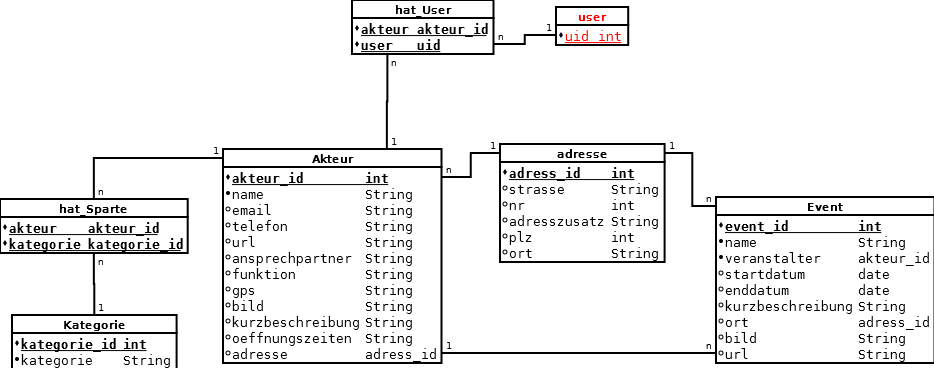
\includegraphics[width=\textwidth]{Datenmodell2.png}\\\\
Wir speichern die Daten in einer relationalen Datenbank, da uns dies eine Einarbeitung in andere Modelle erspart und so zu einer z\"ugigeren Entwicklung f\"uhrt.
\section{Testkonzept}
Um in der Implementierungsphase effizient arbeiten zu k\"onnen, d\"urfen die Tests selbst nicht unn\"otig viel Zeit in Anspruch nehmen. Da ein gro{\ss}er Teil des Teams weder Erfahrung mit Drupals Test-Modul, noch mit Softwaretests im allgemeinen hat und daher extra geschult werden m\"usste, werden nicht alle Teammitglieder Tests durchf\"uhren. Stattdessen werden die im folgenden erl\"auterten Tests von den am Backend arbeitenden Mitgliedern ausgef\"uhrt, die das zu testende Material selbst geschrieben haben.
\subsection{Komponententests}
Bei der Implementierung einzelner Komponenten (Module) ist es wichtig, diese auf Funktionalit\"at und Sicherheit zu testen. Auch wenn wir viel mit bereits vorhandenen Drupalmodulen realisieren werden, sollte jedes einzelne Modul noch einmal gepr\"uft werden. Nur dadurch ist ein einwandfreies Funktionieren gesichert. Tests werden in Testprotokollen dokumentiert, um allen Output festzuhalten und \"Anderungen nachvollziehen zu k\"onnen. F\"ur die Komponententests benutzen wir das interne Drupalmodul \glqq Testing\grqq{}, sowie manuelle Tests. \\
Bisher wurden alle Komponenten manuell getestet. Dies liegt daran, dass erst in der letzte Woche \"uberhaupt zu testende Komponenten implementiert wurden.
\subsection{Integrationstests}
Auch wenn alle Komponenten richtig funktionieren kann es zu Schwierigkeiten beim Zusammenwirken kommen. Es ist daher wichtig, bei dem Einf\"ugen einer Komponente deren Zusammenspiel mit bereits implementierten Komponenten zu testen. Dies wird ebenfalls protokolliert und mittels \glqq Testing\grqq{} gepr\"uft.\\
Bisher wurden alle Integrationstests manuell durchgef\"uhrt. Dies liegt daran, dass erst in der letzte Woche \"uberhaupt zu testende Komponenten implementiert wurden, welche anschlie{\ss}end integriert wurden.
\subsection{Systemtests}
Nach allen Komponententests und Integrationstests muss abschlie{\ss}end das Gesamtsystem gepr\"uft werden. Es wird getestet, ob das Produkt innerhalb der sp\"ateren Nutzungsumgebung funktioniert. F\"ur immer gleiche Anfragen benutzen wir das Tool \glqq Selenium\grqq{}, welches auch bereits in dem Modul \glqq Testing\grqq{} integriert ist. Dieses automatisiert Browseranfragen und gestattet auch Stresstests, da beliebig viele Anfragen auf einmal gestellt werden k\"onnen. Auch das wird protokollarisch festgehalten.\\
Im Rahmen des Hauptprojekts wurden bisher lediglich manuelle Systemtests auf dem Praktikumsserver durchgef\"uhrt. Tests auf dem Server von Matthias Petzold sind jedoch bereits f\"ur die nahe Zukunft geplant.
\section{Glossar}
Stadtteilplattform: \\Eine interaktive (Online)-Plattform, welche der Organisation, Versch\"onerung, Attraktivit\"at, Vermittlung, \glqq News-Verbreitung\grqq{} und vielem mehr dienen soll. Die Plattform sollte so aufgesetzt sein, dass sie in gewisser Weise selbst fuktioniert und mit Inhalten bespielt wird. Das hei{\ss}t Nutzer k\"onnen sich registrieren, f\"ur im Viertel aktive Akteure \"offentliche Profile anlegen und \"uber diese Veranstaltungen und Angebote ver\"offentlichen, ohne dass alles von einem Betreiber der Seite im Voraus einzeln kontrolliert werden muss. Aus inhaltlichen, gesetzlichen, datenschutzrechtlichen Gr\"unden kann eine Nachmoderation, siehe \glqq Nutzer\grqq{}/\glqq Seitenbetreiber\grqq{}). Ziel der Plattform ist es, eine \"ubersichtliche Website zu gestalten, die mittels Interaktiver Karte, Kalender, etc. den Stadtteil mit seinen Akteuren attraktiv macht.

Nutzer:\\Nutzer sind zun\"achst jegliche Besucher der Plattform, die diese zu Informations- und Pr\"asentationszwecken nutzen. Auch alle anderen auf der Plattform aktiven Menschen (z.B. von Betreiberseite) k\"onnen zus\"atzlich in der Rolle des Nutzer auf ihr unterwegs sein. Nutzer k\"onnen alle \"offentlichen Seiten der Plattform aufrufen.\\ 
Nutzer haben zus\"atzlich die M\"oglichkeit, sich auf der Plattform mit einem eigenen Account zu registrieren. Dies erm\"oglicht ihnen das Anlegen eines \"offentlichen Profils f\"ur einen im Stadtteil aktiven Akteur, den der Nutzer auch im realen Leben vertritt. Dies muss im Zweifelsfall von den Seitenbetreibern \"uberpr\"uft und verifiziert werden.

Akteur:\\
Unter Akteuren sind zun\"achst Folgende zu verstehen: Veranstalter, Vereine, Initiativen und Privatpersonen, die im Leipziger Osten auf verschiedene Art aktiv sind. Im Rahmen der Architektur unserer Plattform bezeichnet \glqq Akteur\grqq{} auch die Repr\"asentation einer solchen Institution, die online von einem oder mehreren Nutzern, die der Institution auch in der realen Welt angeh\"oren, (Akteursinhaber \& Akteursmitglieder) vertreten und verwaltet wird. Die \"offentliche Repr\"asentation eines Akteurs auf der Plattform ist das zugeh\"orige Akteursprofil.

Akteursinhaber/Akteursadmin:\\Registrierter Nutzer, der f\"ur einen realweltlichen Akteur ein \"offentliches Profil auf der Stadtteilplattform anlegt, und f\"ur dieses Administratorrechte besitzt. Diese umfassen vollst\"andige Bearbeitungsrechte f\"ur die Inhalte des Profils (ausgenommen Moderation von Nutzerkommentaren), sowie das Recht die L\"oschung des Profils vorzunehmen, bzw. zu veranlassen, oder den Adminstatus an einen anderen registrierten Nutzer oder die Plattformbetreiber abzugeben.

Akteursmitglied:\\Das \"offentliche Profil eines Akteurs soll auch von mehreren Personen verwaltbar sein. Akteursmitglieder sind registrierte Nutzer, denen vom Akteursadmin beschr\"ankte Bearbeitungsrechte zugewiesen wurden. Diese k\"onnen beispielsweise die Bearbeitung von (bestimmten) Inhalten einschlie{\ss}en, aber Akteursmitgliedern keine L\"oschung des Profils zu erm\"oglichen.

Akteursprofil / Kurzdarstellung:\\Von Nutzern verwaltete Selbstdarstellung von Akteuren auf der Stadtteilplattform, \"ahnlich eines Profils in sozialen Netzwerken. Dieses sollte mindestens folgende Daten umfassen: Name, Beschreibung, Adresse, sonstige Kontaktm\"oglichkeit (E-Mail, Facebook...), Sparte, Zielgruppe. Optional sind Bilder, etc. Um ein Profil f\"ur einen Akteur auf der Plattform anzulegen, ben\"otigen die ihm zugeh\"origen Nutzer eine entsprechende Zugangsm\"oglichkeit \"uber einen registrierten Account.

Seitenbetreiber:\\Inhaber und Betreiber der Stadtteilplattform, insbesondere nach \"Ubergabe des Projekts. Der Seitenbetreiber kann eine Person oder eine Institution, z.B. ein Verein sein. In der Praxis k\"onnen im Seitenbetreiber auch verschiedene administrative Aufgaben vereint sein, beispielsweise technische Administration, Nutzerverwaltung, sowie Moderation und redaktionelle T\"atigkeiten. Eine andere personelle und inhaltliche Verteilung der administrativen Aufgaben ist ebenfalls denkbar.

Redakteure:\\Registrierter Nutzer, welcher Schreibrecht f\"ur das Journal besitzt und dort Artikel ver\"offentlichen kann.

Journal:\\Blog, welcher von Redakteuren bearbeitet werden kann.

\end{document}
